\section{Diagram Alir}

Metode pengembangan akselerator perangkat keras untuk \ac{RL} pada penelitian tugas akhir ini dapat dirangkum pada diagram alir pada gambar \ref{fig:flowchart-pengembangan}.

\begin{figure}[h]
	\centering
	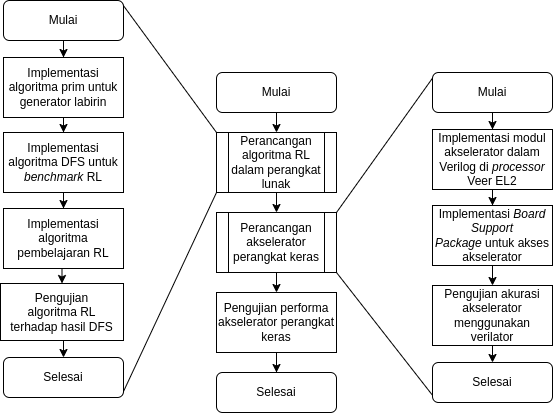
\includegraphics[width=1\textwidth]{chapter-3/flowchart.png}
	\caption{Diagram alir pengembangan akselerator perangkat keras}
	\label{fig:flowchart-pengembangan}
\end{figure}

Pengembangan akselerator perangkat keras secara garis besar, seperti terangkum pada gambar \ref{fig:flowchart-pengembangan}, terdiri dari tiga tahap: perancangan algoritma pada perangkat lunak dan perancangan akselerator perangkat keras. Masing-masing tahapan tersebut akan dijelaskan secara detail pada sub-bab \ref{sec:perancangan-perangkat-lunak} dan \ref{sec:perancangan-akselerator}.
